Adsorption strengths of H on anion-terminated (000$\overline{1}$) surfaces of pure and doped wurtzite ZnO are investigated under varying H surface coverage conditions. Consistent with the prediction of the classical electron counting rules, a $\frac{1}{2}$ \ac{ML} of adsorbed H changes the electronic structure of pure ZnO (000$\overline{1}$) surface from metallic to semiconductor state by saturating unpaired electrons of surface oxygen atoms. This closed-shell electron configuration of ZnO (000$\overline{1}$) surface significantly reduces the adsorption strengths of subsequent H atoms, making the dissociative adsorption of a hydrogen molecule endothermic. A simple electron counting model is applied to predict and tune the coverage-dependent H adsorption strengths on general polar semiconductor surfaces. This model is confirmed by our investigations of H adsorption on (000$\overline{1}$) surfaces of ZnO with a series of dopant elements (Na, Mg, Al, Ti, Fe, Sn, etc.). It can also be applied to H adsorption on other similar polar semiconductors, such as ZnO (000$\bar{1}$) containing O vacancies, wurtzite GaN  (000$\overline{1}$), and zincblende ZnS ($\overline{1}$$\overline{1}$$\overline{1}$) surfaces.

\section{Introduction}

H adsorption on solid surfaces is critical to determine the electronic \cite{pearton2010recent,friend1987electronic}, optical \cite{lee2003electrical,major1986effect}, catalytic \cite{xie2011control,haruta1989gold,levy1973platinum} and many other material applications based on surface physical and chemical properties. For example, the catalytic activities of noble metal catalysts depend on the adsorption strength of critical reaction intermediates on noble metal surfaces at steady states \cite{qi2012adsorbate}. The surface electronic structures of oxides, such as ZnO, can change significantly with different surface coverage of H atoms, and there are still debates on whether the origin of the n-type ZnO conductivity results from adsorbed H on ZnO surfaces \cite{janotti2009fundamentals}. In addition, semiconductor oxides are used as the substrate materials for the metallic thin films, whose adhesion strengths on these substrates can be reduced significantly because of adsorbed H on substrate surfaces, resulting in thin-film dewetting and the formation of the undesired discontinued islands \cite{lin2007density,duriau2006growth}.

There have been many theoretical studies based on first-principles calculations to investigate H adsorption on both metal and oxide surfaces.  The adsorption strengths of H and other adsorbates on surfaces depend not only on the interaction between the surface and a single adsorbed atom/molecule but also the lateral interactions between adsorbates. Usually, the lateral interactions are relatively strong for adsorbates with relatively large atomic sizes, such as oxygen (O), hydroxyl (OH) and carbon monoxide (CO) \cite{Miller09,qi2012adsorbate}. It is excepted that H atoms have relatively weak lateral interactions. First-principles calculations confirmed that H adsorption strength increases slightly and continuously when H surface coverage $\theta_{\textup{H}}$ increases from 0 \ac{ML} to 1 \ac{ML} on metal surfaces \cite{pallassana1999theoretical}. Thus, H coverage on metal surfaces at equilibrium conditions change smoothly with H chemical potential in the reservoir, and Langmuir model can be used to describe the adsorption isotherm of H atoms in many circumstances \cite{Benard01}.

On semiconductor surfaces, the coverage-dependent H adsorption strengths may show different characteristics compared to those on metal surfaces. H coverage on these semiconductor surfaces at equilibrium conditions can change discontinuously by varying H chemical potential in the reservoir. Surface phase diagrams of H adsorption are applied to describe the stable surface structure with different H coverage \cite{deWalle02GaN,wang2005hydrogen,lauritsen2011stabilization}. Clean semiconductor surfaces contain unpaired electrons in dangling chemical bonds and can be energetically unstable \cite{Harrison79, dulub2003novel,wander2001stability,hellstrom2017surface,calzolari2013dipolar}. These surfaces can be stabilized by either surface reconstructions or adsorptions under different environmental conditions \cite{Kaxiras87, meyer2004first,lauritsen2011stabilization,wahl2013stabilization,valtiner2009temperature,Jacobs16ZnO}, and the electron counting rule \cite{pashley1989electron} plays an important role. Recently, a simple electron counting model is developed to predict and study the half-Heusler surfaces of CoTiSb \cite{kawasaki2018simple}. Similarly, the electron counting rule can also be applied to H adsorptions on semiconductor surfaces. So far many surface phase diagrams were obtained case-by-case using first-principles calculations. Most of the reported unreconstructed surfaces with lowest energies \cite{meyer2004first,valtiner2009temperature,Jacobs16ZnO} still follow the electron counting rule. Based on the understanding of the electron counting rule, it is easy to predict equilibrium H coverage on a given surface construction. However, a general method to manipulate H surface coverage is still missing.

Many efforts have been made to study H adsorption on surfaces of ZnO \cite{Meyer03,meyer2004first,wang2005hydrogen,valtiner2009temperature,lauritsen2011stabilization, wahl2013stabilization, Jacobs16ZnO}, a wide-band-gap semiconductor widely used in the fields of catalysis, gas sensing, and optoelectronics \cite{Ozgur05_ZnO,Klingshirn07_ZnO}. There are also a few studies on surfaces of ZnO with dopant elements, like Al and Mg \cite{lin2009first, lahmer2015effect}. Since there are increasing applications of doped ZnO and other semiconductors depending on their surface structures and electronic properties \cite{Pan08_doped_ZnO, Georgekutty08_Ag_ZnO, lin2009first, Ling11_Sn-Doped, Buonsanti11_Al_ZnO, Kim14_doped, Hsu14_Ag_ZnO, Lin17_Ni_SnO2}, it is necessary to explore the general principles that guide H adsorption strengths on a wide range of pure and doped ZnO and similar semiconductor surfaces. Especially, it will be interesting to verify for these general cases the accuracy of the electron counting model, which was recently applied to determine the atomic and electronic structures of (001) surface of CoTiSb, a prototypical semiconducting half-Heusler compound \cite{kawasaki2018simple}.

When ZnO bulk structure is chopped into slabs along [0001] directions, two types of surfaces, O-terminated (000$\overline{1}$) surface and Zn-terminated  (0001) surface, are exposed as shown in Fig. \ref{Chap:ZnO_H:fig:ZnO}. These two surfaces were found to have different stabilization principles\cite{lauritsen2011stabilization}: the Zn-terminated  (0001) surface usually has corrugated morphology and complex surface reconstructions because the transition-metal element Zn is more flexible with respect to bonding orientation \cite{dulub2003novel,woll2007chemistry}; the O-terminated (000$\bar{1}$) surface is usually flat on the top layer with different coverage and occupation sites for O and H atoms depending on their chemical potentials because O prefers the bonding configurations with certain bond angles and nearest neighbors \cite{meyer2004first,lauritsen2011stabilization}. In addition, many functional applications of ZnO surfaces are used in oxygen-rich environments, where there are few oxygen vacancies on ZnO (000$\bar{1}$) surface \cite{meyer2004first,lauritsen2011stabilization,wahl2013stabilization}. For these reasons, we use the simple O-terminated (000$\bar{1}$) wurtzite ZnO by its bulk-terminated ideal form (the top surface in Fig. \ref{Chap:ZnO_H:fig:ZnO}) as the model system to investigate the effects of electronic structures and dopant elements on the coverage-dependent H adsorption strength in this study.

\section{Coverage-dependent Hydrogen Adsorption Energies on ZnO (000$\bar{1}$) Surface}
\label{sec:Hcoverage}
\begingroup
\begin{figure}[!ht]
  \centering
  \subfigure[]{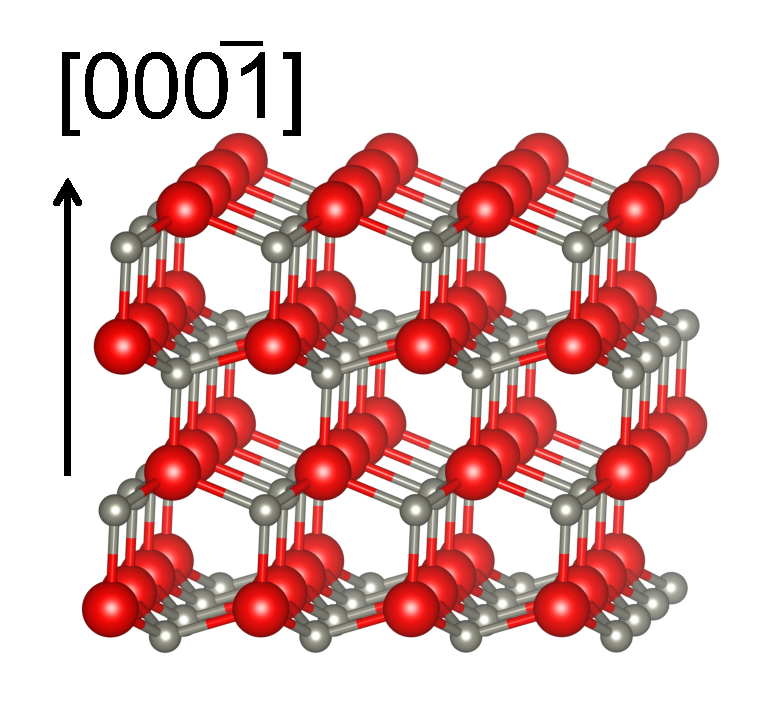
\includegraphics[width=0.4\linewidth]{Chap1/polar1.pdf}}\label{Chap:ZnO_H:fig:ZnO}
  \subfigure[]{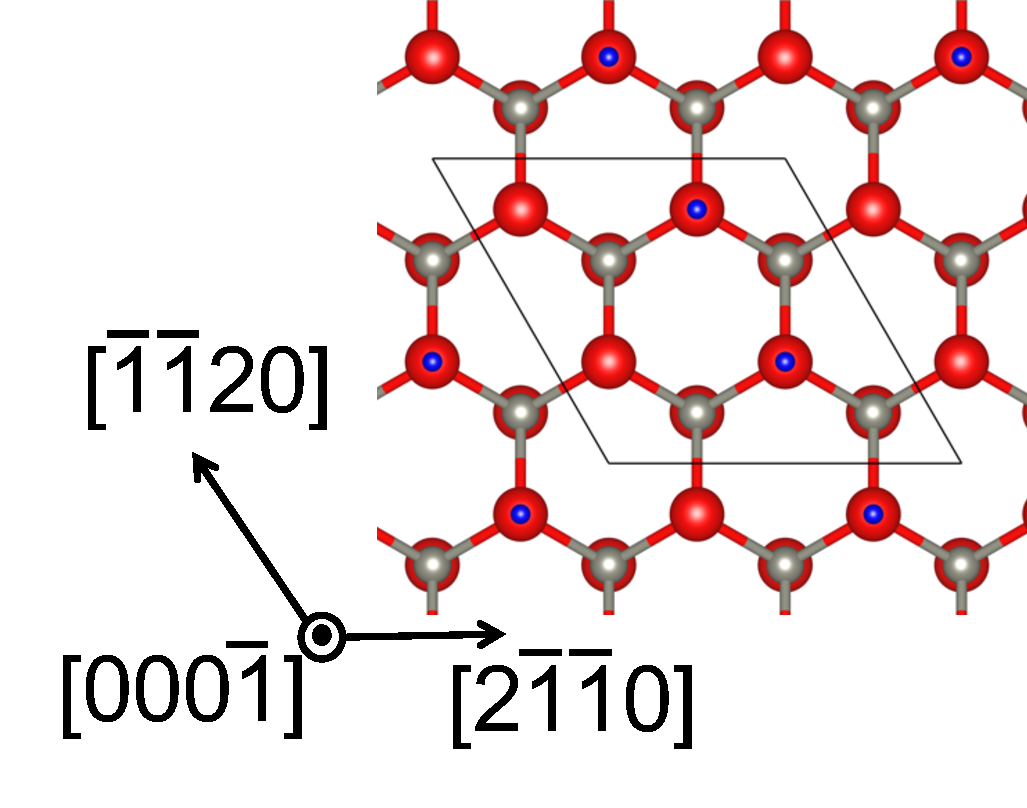
\includegraphics[width=0.4\linewidth]{Chap1/surface2x2.pdf}}\label{Chap:ZnO_H:fig:ZnOSurf}
\caption[Schematic of (2$\times$2) supercell used to model  (000$\bar{1}$) wurtzite ZnO surface with H adsorption.]{(a) and (b): Schematic of (2$\times$2) supercell used to model  (000$\bar{1}$) wurtzite ZnO surface with H adsorption. Large red, small grey and small blue atoms are O, Zn and H atoms, respectively. (a) is the side view projection of ZnO (000$\bar{1}$) slabs, (b) is the top view of (2$\times$2) O-terminated (000$\bar{1}$)  ZnO surface with $\frac{1}{2}$ ML adsorbed H.}
\label{fig1}
\end{figure}
\endgroup

We performed first-principles calculations based on \ac{DFT} by using \ac{VASP} \cite{kresse1996efficient,kresse1999ultrasoft}. Projector augmented wave (PAW) \cite{blochl1994projector} potentials with Perdew-Burke-Ernzerhof (PBE) \cite{perdew1996generalized} exchange-correlation functional and the Hubbard U correction \cite{dudarev1998electron} were used. We applied GGA+U with $U_\text{eff}=U - J = 5.0 eV$ on Zn \textit{d} orbitals as reported in literature\cite{huang2012detailed, oba2010native}. Several other Hubbard U correction parameters ($\text{U}_\text{eff} =$ 3.0 or 7.5 eV) were also tested and showed no significant effects on H adsorption energies. K-points sampling for Brillouin zone integration was performed on a grid of 6$\times$6$\times$1, 6$\times$4$\times$1 with Monkhorst-Pack meshing scheme for (2$\times$2) and (2$\times$3) surface, respectively\cite{monkhorst1976special}. An energy cut-off of 450.0 eV was used in the calculation. The electronic convergence threshold was set as $10^{-4}$ eV. The wurtzite ZnO (000$\overline{1}$) surfaces were constructed by periodic supercell slab models. (2$\times$2) supercells with a vacuum layer of 18 $\angstrom$ in the directions perpendicular to the surfaces were applied as shown in Fig. \ref{Chap:ZnO_H:fig:ZnO} and \ref{Chap:ZnO_H:fig:ZnOSurf}. Each slab contains eight layers of Zn-O repeating units along [0001] direction. Since the ZnO surface slab supercell is not symmetric along [0001] direction, we tested the dipole effects on H adsorption energies and found the dipole effects are minimal if the passivation of the Zn-terminated surface eliminates the artificial electron transfer described as the following. So only the results corresponding no dipole corrections are reported in this study.

As shown in Fig. \ref{Chap:ZnO_H:fig:ZnO}, two types of surfaces are exposed, O-terminated (000$\overline{1}$) surfaces and Zn-terminated  (0001) surfaces, are presented in ZnO slab by its bulk-terminated ideal form. In theoretical modeling, if both sides of a surface slab layer are exposed without modifications, there will be unbalanced electron transfer from Zn-terminated surface to O-terminated surface\cite{Meyer03}. In reality, if the O-terminated surface is exposed to the external environment, the Zn-terminated surface usually is connected to a substrate, which can act as an electron reservoir and compensate unsaturated electrons on the Zn-terminated surface. Many methods have been applied to reduce this artificial electron transfer, such as the introduction of pseudo-hydrogen passivation atoms, Zn vacancies and other adsorbates on Zn-terminated surfaces\cite{calzolari2013dipolar,lin2007microscopic,lahmer2015effect}.

In this work, we focused on O-terminated (000$\overline{1}$) ZnO surface, where H atoms are adsorbed on the top of each surface O atoms as shown in Fig. \ref{Chap:ZnO_H:fig:ZnOSurf}. Zn-terminated (0001) surface on the other side of the slab model was passivated by two different methods to exam their effect on long-distance surface-to-surface electron transfer in the same supercell \cite{zhang2018tuning}. First, $\frac{1}{4}$ ML of Zn vacancy was introduced on the top layer of the Zn-terminated surface in a (2$\times$2) supercell. Second, pseudo-hydrogen atoms with different numbers of valence electrons were introduced on the top layer of the Zn-terminated surface. Each Zn atom on the top layer of the Zn-terminated surface was bonded with one pseudo-hydrogen atom, which can have 1.5, 1.0 or 0.5 electrons (denoted as H$_{1.5}$, H$_{1.0}$ and H$_{0.5}$, respectively). In this paper, all the adsorption energy calculations and electronic structure analyses were conducted on the supercells with H$_{1.5}$-passivated Zn-terminated surfaces unless otherwise specified. The reason will be explained and verified in App. \ref{appd:passivation}.

In this paper, hydrogen adsorption energy $E_{\textup{ad}}^{\textup{H}}$ with H surface coverage $\theta_{\textup{H}}$ equal to $\frac{n}{m}$ ML is calculated as:
\begin{equation}
  \begin{array}{rcl}
       E_{\textup{ad}}^{\textup{H}}(\theta_{\textup{H}}=\frac{n}{m} \textup{ML})&=&E_{\textup{slab+}n\textup{ H}}-E_{\textup{slab+}(n-1) \textup{ H}}-\frac{1}{2}E_{\textup{H}_{2}}
  \end{array}
  \label{eq1}
\end{equation}
Here $E_{\textup{slab+}n \textup{H}}$ and $E_{\textup{slab+}(n-1) \textup{H}}$ is the total energy of surface slab supercell containing $n$ and $n-1$ adsorbed H atoms, respectively, and $E_{\textup{H}_{2}}$ is the energy of an isolated H$_2$ molecule. The ($x\times y$) surface slab supercell itself contains $m=x\cdot y$ duplicates of (1$\times$1) unit cell of 2D surface lattice, so $m=4$ and $m=6$ for (2$\times$2) and (2$\times$3) slab supercells, respectively. As shown in Fig. \ref{Chap:ZnO_H:fig:Ead}, $E_{\textup{ad}}^{\textup{H}}$ on platinum (Pt) (111) surface only increases slightly with a rising surface H coverage $\theta_{\textup{H}}$ ($\delta E_{\textup{ad}}^{\textup{H}}$ $\sim0.1$ eV when  $\theta_{\textup{H}}$ increases from $\frac{1}{4}$ ML to 1 ML ). On the contrary, $E_{\textup{ad}}^{\textup{H}}$ is highly negative and increases slightly on (2$\times$2) slab supercell of (000$\overline{1}$) ZnO when  $\theta_{\textup{H}}$ = $\frac{1}{4}$ and $\frac{1}{2}$ ML, then $E_{\textup{ad}}^{\textup{H}}$ jumps up suddenly after $\theta_{\textup{H}}$ above $\frac{1}{2}$ ML. 

\begingroup
\begin{figure}[!ht]
  \centering
  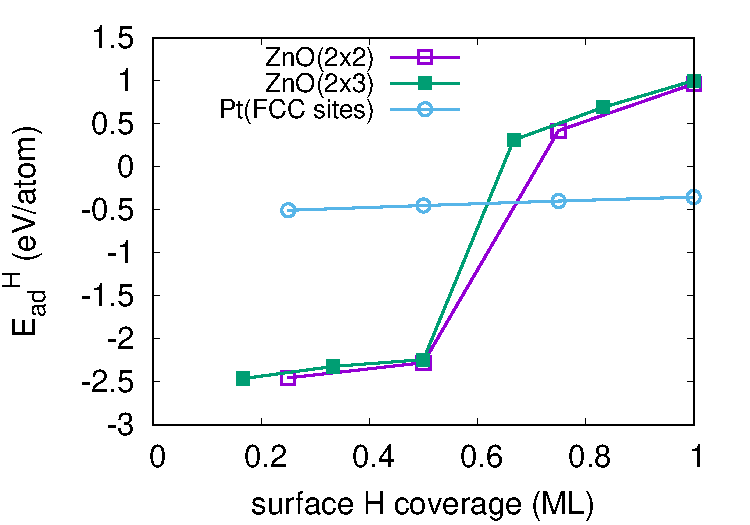
\includegraphics[width=0.75\linewidth]{Chap1/Eadh_coverage_H.pdf}
\caption[H adsorption energies on ZnO surfaces with different H coverage]{H adsorption energies $E_{\textup{ad}}^{\textup{H}}$ defined by Eq. \ref{eq1} on ZnO (000$\overline{1}$) and Pt (111) surfaces with different H coverage}
  \label{Chap:ZnO_H:fig:Ead}
\end{figure}
\endgroup

In order to confirm the critical transition, $E_{\textup{ad}}^{\textup{H}}$ for a larger wurtzite ZnO (000$\overline{1}$) slab supercell with (2$\times$3) in-plane periodicity was also studied. The abrupt increase of $E_{\textup{ad}}^{\textup{H}}$, again, happens when $\theta_{\textup{H}}$ is higher than $\frac{1}{2}$ ML, as shown in Fig. \ref{Chap:ZnO_H:fig:Ead}. It can be concluded that there is a large driving force ($E_{\textup{ad}}^{\textup{H}}$ $<$ -2 eV per H atom) for an isolated H$_2$ molecule to dissociate into two H atoms adsorbed on ZnO (000$\overline{1}$) surface if $\theta_{\textup{H}}$ smaller than $\frac{1}{2}$ ML, above which such adsorption-dissociation reaction becomes highly endothermic and difficult to occur ($E_{\textup{ad}}^{\textup{H}}$ $>$ 0). These results are consistent with previous theoretical calculations and experimental characterizations that $\frac{1}{2}$ ML of adsorbed H were often observed on ZnO (000$\overline{1}$) surface\cite{lin2007density,meyer2004first,lauritsen2011stabilization}.

\section{Electronic Structure Analyses and Electron Counting Model}

Electronic structures of surface oxygen atoms before and after H adsorption are analyzed in order to understand the mechanism to determine the critical transition of $E_{\textup{ad}}^{\textup{H}}$ on ZnO (000$\overline{1}$) surface. We plot \ac{PDOS} of all four surface O atoms on the top layer of (2$\times$2) ZnO (000$\overline{1}$) surface with different H coverage in Fig. \ref{Chap:ZnO_H:fig:DOSO}. \ac{PDOS} of O atoms for $\theta_{\textup{H}}$ = 0 ML and $\frac{1}{4}$ ML cases have strong peaks at the Fermi level, so these ZnO surfaces are in metallic states. When ZnO surface is covered by $\frac{1}{2}$ ML of H atoms, the Fermi level is 0.1 eV above valence band maximum, making these ZnO surfaces in semiconductor states. The cases of  $\theta_{\textup{H}}$ = $\frac{3}{4}$ and 1 ML keep in semiconductor states by further decreasing the valence band maximum to the positions much lower than the Fermi level. \ac{PDOS} of all surface atoms, including all O, Zn and adsorbed H atoms on the top layer of ZnO (000$\overline{1}$) surface, are plotted in Fig. \ref{Chap:ZnO_H:fig:DOSall} to confirm the above analyses. Similar to Fig. \ref{Chap:ZnO_H:fig:DOSO},  \ac{PDOS} of all surface atoms for the cases of $\theta_{\textup{H}}$ =  0 ML and $\frac{1}{4}$ ML show strong peaks in the Fermi level, while the \ac{PDOS} of all surface atoms for the cases of $\theta_{\textup{H}}=\frac{1}{2}$ ML and above exhibit semiconductor characteristics. Thus,  $\frac{1}{2}$ ML is the critical $\theta_{\textup{H}}$ to transform  ZnO (000$\overline{1}$) surface from metallic into semiconductor states. 

\begingroup
\begin{figure}[!ht]
  \centering
  \subfigure[]{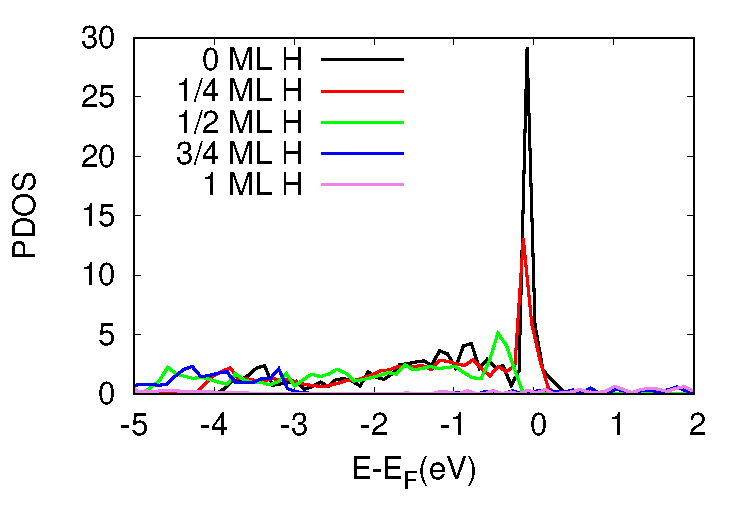
\includegraphics[width=0.45\linewidth]{Chap1/DOS_ZnO_surfO.pdf}}\label{Chap:ZnO_H:fig:DOSO}
  \subfigure[]{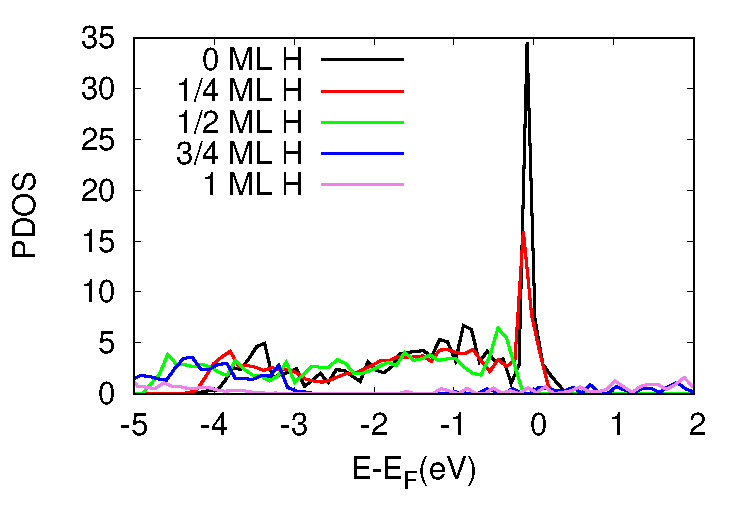
\includegraphics[width=0.45\linewidth]{Chap1/DOS_ZnO_surface_all.pdf}}\label{Chap:ZnO_H:fig:DOSall}
  \caption[\ac{PDOS} for all the surface O atoms on pure ZnO (2$\times$2) (000$\overline{1}$) surface under different H coverage]{(a) \ac{PDOS} for all the surface O atoms on pure ZnO (2$\times$2) (000$\overline{1}$) surface under different H coverage. (b) \ac{PDOS} of all O, Zn and adsorbed H atoms on the topmost layer of ZnO (000$\overline{1}$) surface under different H coverage.}
  \label{Chap:ZnO_H:fig:DOS}
\end{figure}
\endgroup

The coincidence ($\frac{1}{2}$ ML) of the critical $\theta_{\textup{H}}$ for the abrupt change of $E_{\textup{ad}}^{\textup{H}}$ and the critical $\theta_{\textup{H}}$ for the metal-semiconductor transition indicates that $E_{\textup{ad}}^{\textup{H}}$ is controlled by surface electronic structures. This coincidence can be explained by the electron counting model\cite{pashley1989electron}. Each Zn has 2 valence electrons, and each O has 6 valence electrons. In bulk wurtzite lattice, each Zn/O atom connects to 4 nearby O/Zn atoms so that every Zn-O bond has 2 valence electrons, in which 1.5 electrons are contributed from O and 0.5 electron is from Zn. After bulk ZnO is chopped into two slabs with two surfaces in [0001] direction, each surface O and Zn atom has one broken Zn-O bond, as shown in Fig. \ref{Chap:ZnO_H:fig:ZnO}. For Zn-terminated (0001) surface, we applied appropriate methods to passivate the dangling bonds as explained in App. \ref{appd:passivation}. For O-terminated (000$\overline{1}$) surface, each O atom requires 0.5 more electron to fill its dangling bond and reach the closed-shell electron configuration. Thus, the electrons of clean O-terminated (000$\overline{1}$) surface are in open-shell configurations. 

The unpaired electrons from surface O atoms are delocalized, making ZnO surface in metallic states. There is a large energetic driving force for surface O atoms to reach closed-shell configurations, meaning ZnO surface has a strong adsorption strength to any atoms/molecules that can contribute electrons to surface O atoms, such as H. In a simple picture, each H atom can contribute one electron to make 2 surface O atoms on (000$\overline{1}$) ZnO surface transform into electron closed-shell configurations. Thus, once $\theta_{\textup{H}}$ reaches $\frac{1}{2}$ ML, there are no unpaired electrons in delocalized states on (000$\overline{1}$) ZnO surface. Correspondingly, the surface transforms into semiconductor state and has much weaker adsorption strength for the consecutive H atoms.

\begingroup
\begin{figure}[!ht]
  \centering
  \subfigure[]{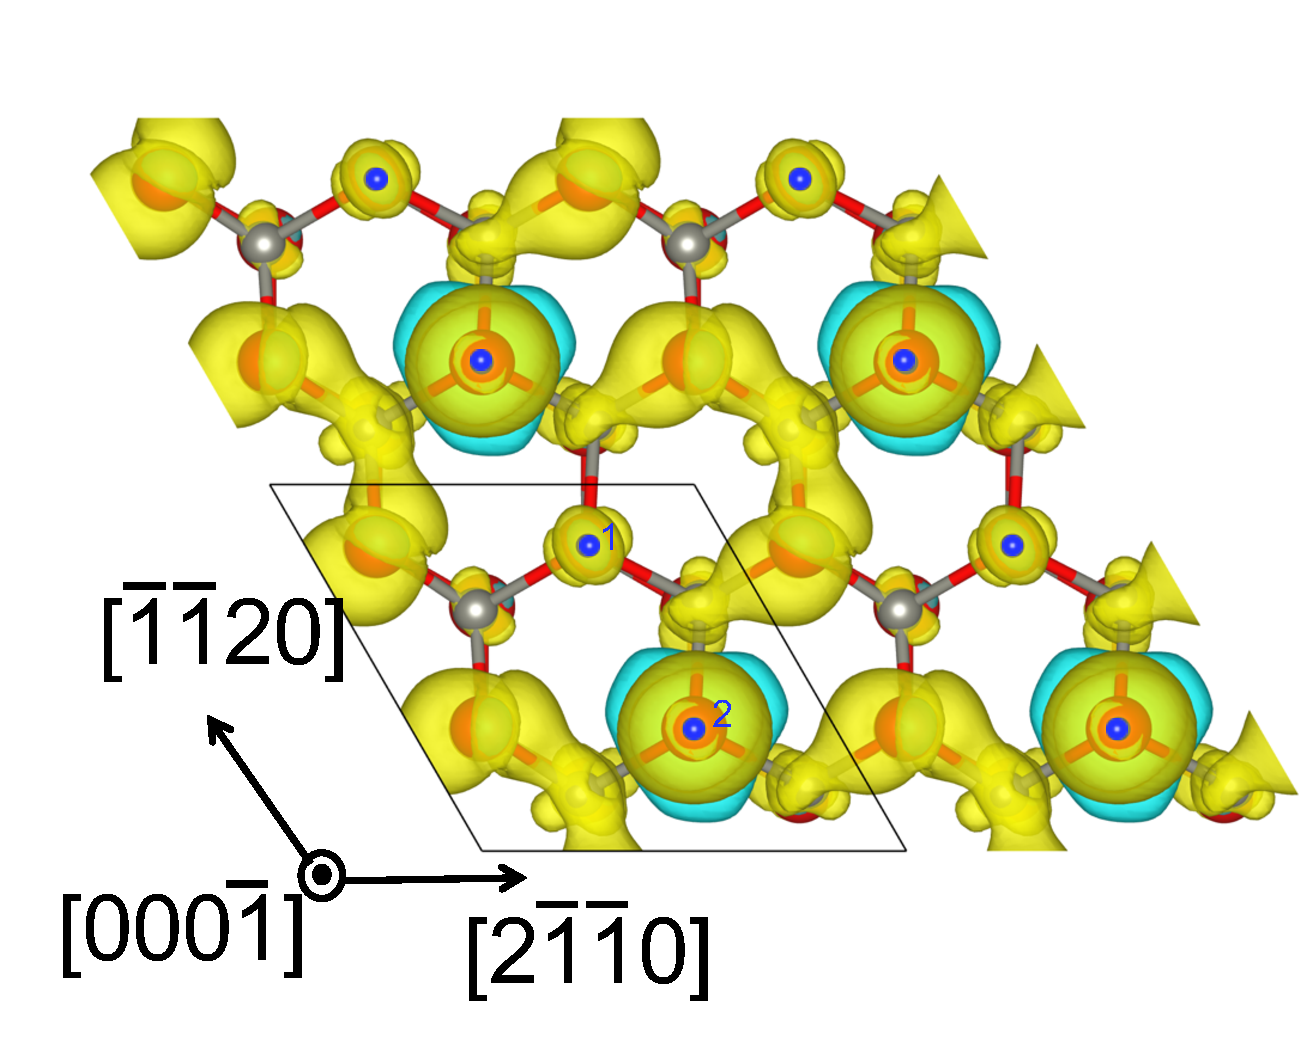
\includegraphics[width=0.49\linewidth]{Chap1/chgdiff1.pdf}}\label{Chap:ZnO_H:fig:chgdiff1}
  \subfigure[]{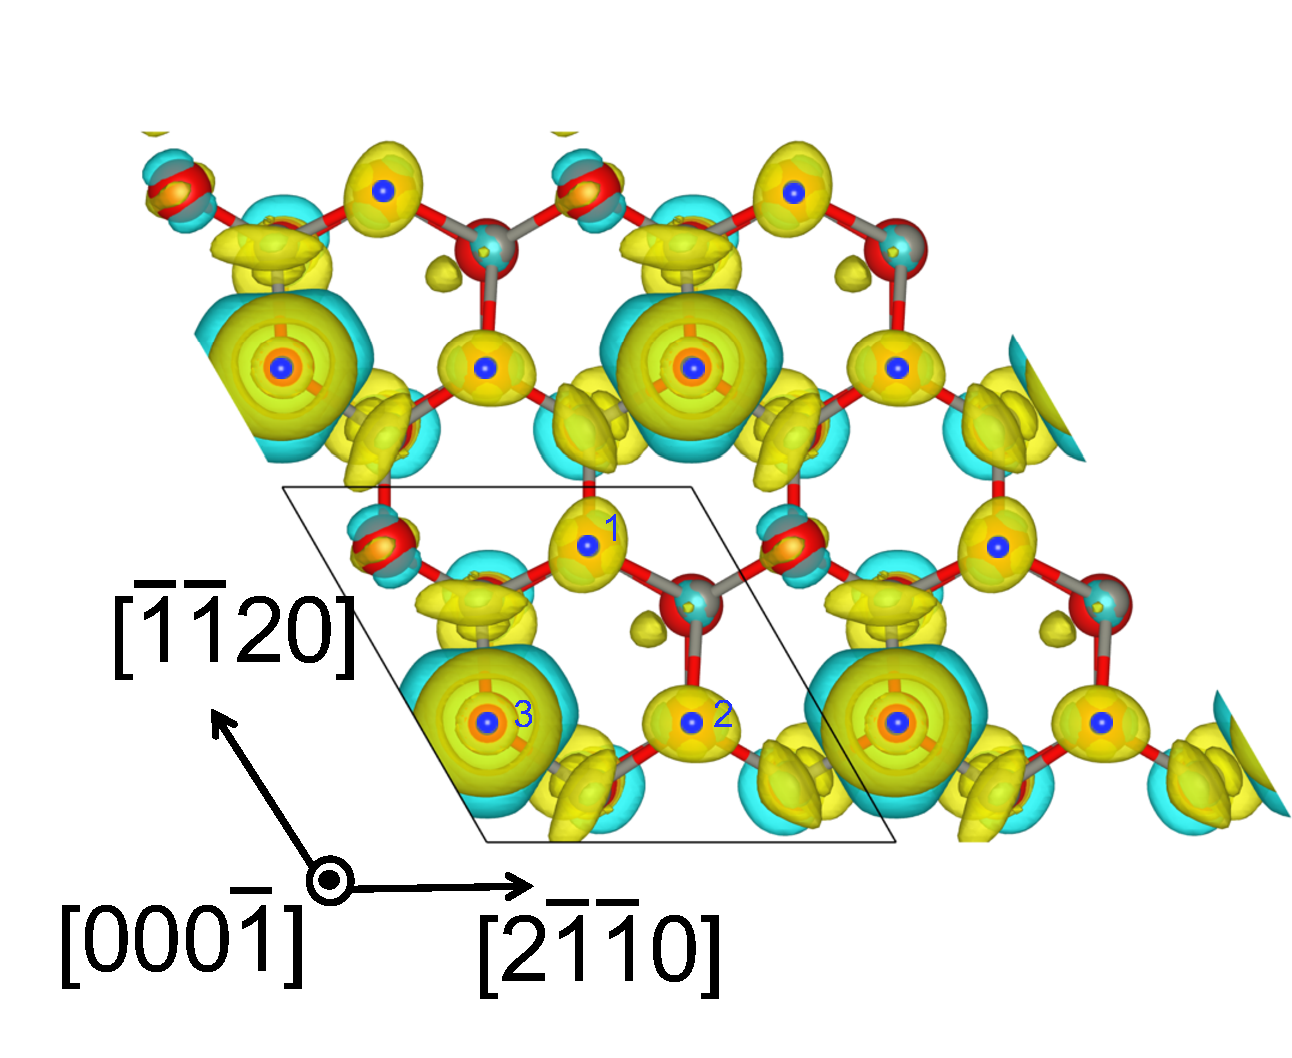
\includegraphics[width=0.49\linewidth]{Chap1/chgdiff2.pdf}}\label{Chap:ZnO_H:fig:chgdiff2}
\caption[Top views of the charge density difference isosurfaces before and after H adsorption]{Top views of the charge density difference isosurfaces before and after (a) the second H and (b) the third adsorption on ZnO (000$\overline{1}$) surface in (2$\times$2) supercells, corresponding to $\Delta\rho(\theta_{\textup{H}}= \frac{1}{2} \textup{ ML})$ and $\Delta\rho(\theta_{\textup{H}}= \frac{3}{4} \textup{ ML})$ defined in Eq. \ref{eq2}, respectively. Large red, small grey and small blue atoms are O, Zn and H atoms, respectively. Label 1, 2 and 3 in the plots denote the adsorption site for the first, second, and third H atom, respectively. The yellow and blue color indicate electron accumulation and annihilation with the isosurface of $0.001e/{\textup{\AA}}^3$.}
  \label{fig3}
\end{figure}
\endgroup

Such electron counting rule and the corresponding \ac{PDOS} analyses can be further confirmed by the analyses of charge density difference on ZnO (000$\overline{1}$) surface due to H adsorption. Here we define the charge density difference $\Delta\rho$ at different $\theta_{\textup{H}}$ as the following
\begin{equation}
  \begin{array}{rcl}
    \Delta\rho(\theta_{\textup{H}}=\frac{n}{m}\textup{ML})&=&\rho(\textup{slab+}n\textup{H})-\rho(\textup{slab+}(n-1)\textup{H})
  \end{array}
  \label{eq2}
\end{equation}
Here $\rho(\textup{slab+}n \textup{H})$ and $\rho(\textup{slab+}(n-1) \textup{H})$ is the charge density of ZnO (000$\overline{1}$) surface slab with $n$ and $(n-1)$ adsorbed H atoms, respectively. For (2$\times$2) supercell, $\Delta\rho(\theta_{\textup{H}}= \frac{1}{2} \textup{ ML})$ and  $\Delta\rho(\theta_{\textup{H}}= \frac{3}{4} \textup{ ML})$ corresponds to the charge density difference induced by the adsorption of the second and third H atom in the supercell, as shown in Fig. \ref{Chap:ZnO_H:fig:chgdiff1} and  \ref{Chap:ZnO_H:fig:chgdiff2}, respectively. 

In Fig. \ref{Chap:ZnO_H:fig:chgdiff1}, the second H added on (2$\times$2) ZnO (000$\overline{1}$) surface induces charge density accumulation not only near this H atom itself but also other surface sites without H. Such delocalized $\Delta\rho$ is consistent with the metallic state of ZnO (000$\overline{1}$) surface with $\theta_{\textup{H}}$ $<$ $\frac{1}{2}$ ML. The increase of charge density at multiple surface sites indicates that the electron from the second H atom intends to saturate the unpaired electrons on the whole surface and induce the metal-semiconductor transition. In Fig. \ref{Chap:ZnO_H:fig:chgdiff2}, the third H added on (2$\times$2) ZnO (000$\overline{1}$) surface results in charge density accumulation mostly located near the third H atom itself, with a localized s-orbital-like isosurface of $\Delta\rho$ shown in Fig. \ref{Chap:ZnO_H:fig:chgdiff2}. Such localized $\Delta\rho$ is consistent with the semiconductor electronic structure of ZnO (000$\overline{1}$) surface with $\theta_{\textup{H}}$ $\geq$ $\frac{1}{2}$ ML. 



\section{Hydrogen Adsorption on (000$\overline{1}$) Surface of ZnO with Dopants}
\label{sec:doped}

In this study, we find that the electron counting model can also be applied to explain the variation of $E_{\textup{ad}}^{\textup{H}}$ with $\theta_{\textup{H}}$ on (000$\overline{1}$) surfaces of doped ZnO\cite{pashley1989electron}. Different metallic elements are added as substitutional dopants on Zn lattice sites. Because these dopant elements can have different numbers of valence electrons than Zn, it can change the required number of adsorbed H atoms to saturate all surface O atoms and induce the metal-semiconductor transition on the surface. Correspondingly, the critical $\theta_{\textup{H}}$ for the transition of $E_{\textup{ad}}^{\textup{H}}$ can also be varied.  Based on this mechanism, one Zn atom in ZnO bulk lattice is replaced by various types of dopant atoms. 

The dopant atoms located at slab layers with different distances to the top (000$\overline{1}$) surface layer are investigated, and our results show that the location of such dopant atom does not have a significant effect on H adsorption energetics and the critical $\theta_{\textup{H}}$. As illustrated in Tab. \ref{tab:layer}, H adsorption energies with the substitutional dopant elements on Zn lattice sites at different layers away from the O-terminated (000$\bar{1}$) surfaces are listed. H adsorption energies do not show significant variations for the dopant atom at varying distances to the top layer of (000$\bar{1}$) surfaces. Thus, the results for one dopant atom (Al, Ti, V, Na, Mg, Be, Fe, Sn, and Pb) at bulk Zn site far away from the top surface layer in (2$\times$2) ZnO (000$\overline{1}$) supercells are summarized in Fig. \ref{Chap:ZnO_H:fig:doped}. 

\begin{table}[!htbp]
\centering
\caption[Comparison of different doping locations to the top surface layer]{The coverage-dependent adsorption energy of H atom $E_{\textup{ad}}^{\textup{H}}$ (unit: eV/atom) on O-terminated  (000$\bar{1}$) ZnO surface with substitutional Be dopant atom at different locations to the top surface layer. Layer 1 is at the Zn lattice site nearest to the top surface layer.}
\label{tab:layer}
\begin{tabular}{lllll}
\hline
eV/atom      & 0.25ML & 0.5ML & 0.75ML & 1ML  \\ \hline
Layer 1      & -2.71  & -2.39 & 0.52   & 0.97 \\
Layer 2      & -2.38  & -2.23 & 0.43   & 0.97 \\
Layer 3      & -2.42  & -2.28 & 0.51   & 0.94 \\
Layer 4      & -2.39  & -2.32 & 0.46   & 0.98 \\\hline
\end{tabular}
\end{table}

\begingroup
\begin{figure}[!htb]
  \centering
  \subfigure[]{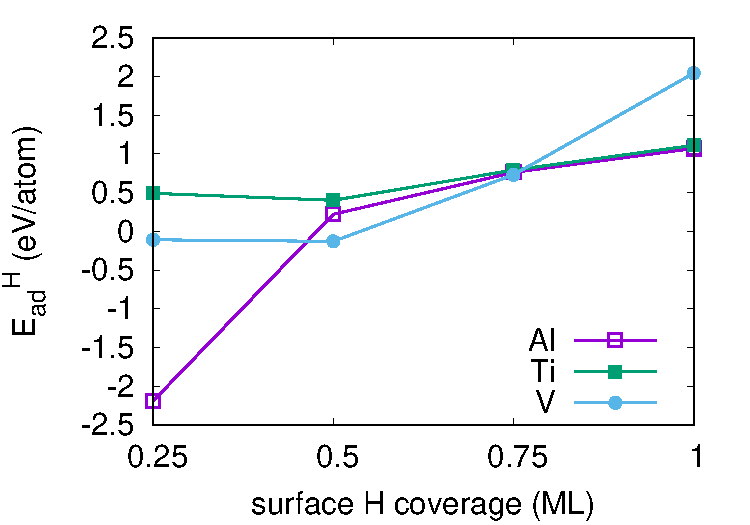
\includegraphics[width=0.32\linewidth]{Chap1/E_C_1.pdf}}\label{Chap:ZnO_H:fig:dop1}
  \subfigure[]{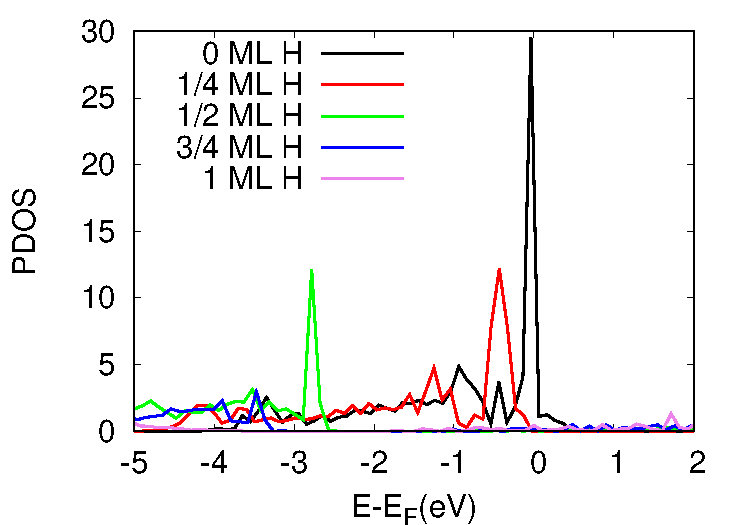
\includegraphics[width=0.32\linewidth]{Chap1/DOS_Al_surfO.pdf}}\label{Chap:ZnO_H:fig:dop2}
  \subfigure[]{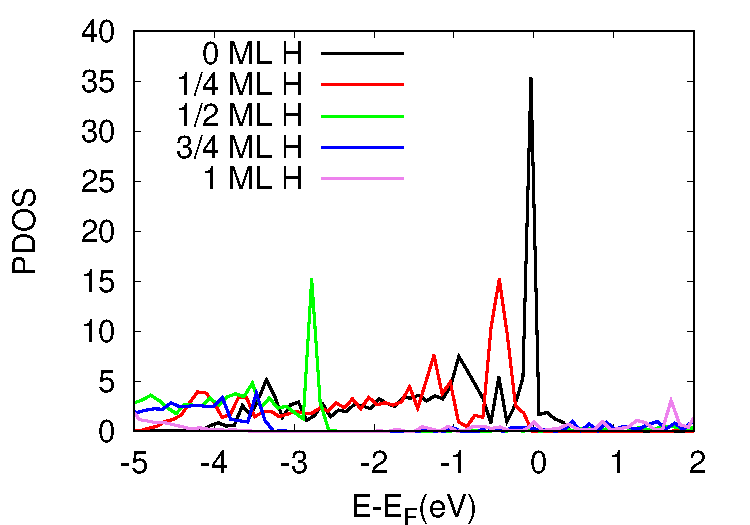
\includegraphics[width=0.32\linewidth]{Chap1/DOS_Al_surf_all.pdf}}\label{Chap:ZnO_H:fig:dop3}
   \qquad
  \subfigure[]{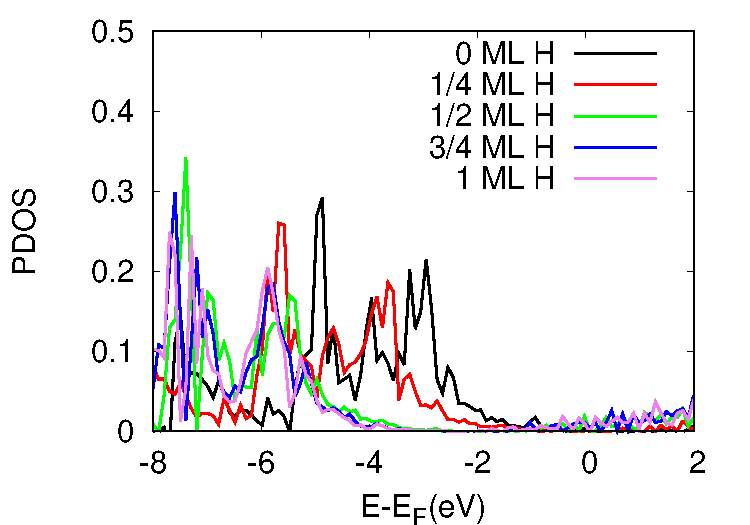
\includegraphics[width=0.32\linewidth]{Chap1/DOS_bulk_Al.pdf}}\label{Chap:ZnO_H:fig:dop4}
  \subfigure[]{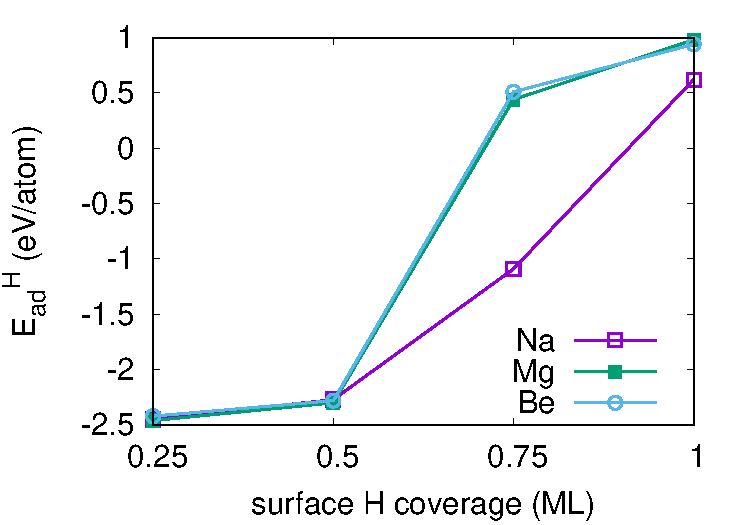
\includegraphics[width=0.32\linewidth]{Chap1/E_C_2.pdf}}\label{Chap:ZnO_H:fig:dop5}
  \subfigure[]{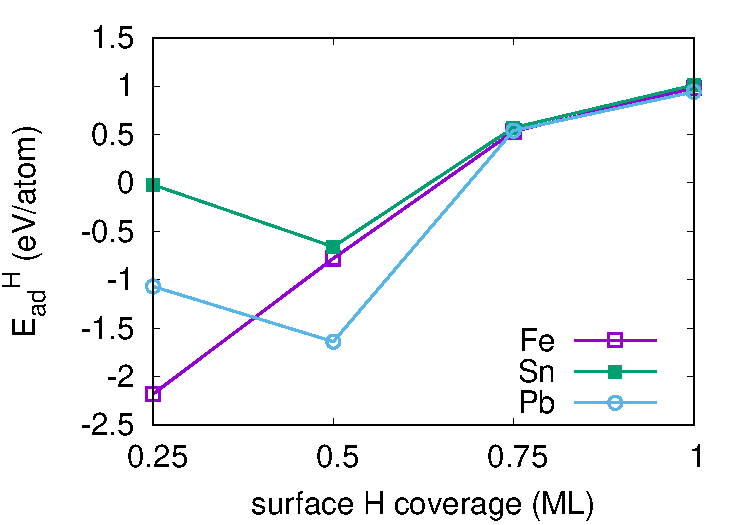
\includegraphics[width=0.32\linewidth]{Chap1/E_C_3.pdf}}\label{Chap:ZnO_H:fig:dop6}
\caption[H adsorptions on ZnO surfaces with different doping]{(a) $E_{\textup{ad}}^{\textup{H}}$ on (2$\times$2) ZnO (000$\overline{1}$) surface with one substitutional dopant atom (Al, Ti or V) at bulk Zn site. Each dopant atom has more valence electrons more than Zn. (b) \ac{PDOS} for all the O atoms on top surface layer of Al-doped ZnO (000$\overline{1}$) under different $\theta_{\textup{H}}$. (c) \ac{PDOS} of all O, Zn and adsorbed H atoms on the topmost layer of Al-doped ZnO (000$\overline{1}$) under different $\theta_{\textup{H}}$. (d) \ac{PDOS} for Al atom in the bulk layer of Al-doped ZnO (000$\overline{1}$) under different $\theta_{\textup{H}}$. (e) $E_{\textup{ad}}^{\textup{H}}$ on (2$\times$2) ZnO (000$\overline{1}$) surface with one substitutional dopant atom (Mg, Be or Na)  at bulk Zn sites. Each dopant atom has equal or less valence electrons than Zn. (f) $E_{\textup{ad}}^{\textup{H}}$ on (2$\times$2) ZnO (000$\overline{1}$) surface with one substitutional dopant atom (Fe, Sn or Pb) at bulk Zn sites. Each dopant atom has multiple common charge states.}
\label{Chap:ZnO_H:fig:doped}
\end{figure}
\endgroup

In Fig. \ref{Chap:ZnO_H:fig:dop1}, all dopant atoms (Al, Ti and V) have more valence electrons than Zn. For Al-doped ZnO surface, if the one extra valence electron from Al already transfers to O atoms on the top surface layer, only one H atom is required to saturate all 4 O atoms in a (2$\times$2) supercell and induce the metal-semiconductor transition according to the electron counting model. Consistent with this interpretation, the H adsorption strength for the Al-doped ZnO surface in Fig. \ref{Chap:ZnO_H:fig:dop1} is as strong as the pure ZnO surface in Fig. \ref{Chap:ZnO_H:fig:Ead} when $\theta_{\textup{H}}$ $\leq$ $\frac{1}{4}$ ML. Above this critical $\theta_{\textup{H}}$, $E_{\textup{ad}}^{\textup{H}}$ suddenly increases to positive values, consistent with the proposed metal-semiconductor transition for ZnO surface. This interpretation is further confirmed by analyses of \ac{PDOS} of all four surface O atoms on (2$\times$2) Al-doped ZnO surface in Fig. \ref{Chap:ZnO_H:fig:dop2}. \ac{PDOS} of O atoms with $\theta_{\textup{H}}$ = 0 ML case have strong peaks at the Fermi level. When Al-doped ZnO surfaces are covered by $\frac{1}{4}$ to 1 ML of H atoms, there are no peaks on the Fermi level, making these surfaces in semiconductor states. \ac{PDOS} of all surface atoms, including all the O, Zn and adsorbed H atoms on the topmost layer of Al-doped ZnO (000$\overline{1}$) surface, are plotted in Fig. \ref{Chap:ZnO_H:fig:dop3} to confirm the above analyses. Similar to Fig. \ref{Chap:ZnO_H:fig:dop2},  \ac{PDOS} of all surface atoms for the case of $\theta_{\textup{H}}$ =  0 ML  show strong peaks in the Fermi level, while \ac{PDOS} of all surface atoms for the cases of $\theta_{\textup{H}}=\frac{1}{4}$ ML and above exhibit semiconductor characteristics. \ac{PDOS} of the Al atom, which is located at the third layer away from the (000$\overline{1}$) O-term surface, under different H surface coverages is also plotted in Fig. \ref{Chap:ZnO_H:fig:dop4}.  As can be seen from the plot, there is no significant peak around Fermi level for all the H surface coverages, showing that the bulk Al atom under different H surface coverages is also saturated in closed-shell electron configuration. Interestingly, \ac{PDOS} of Al downshifts indicating a stronger bonding between Al and nearby O atoms as the H surface coverages increases.

If one Zn atom is replaced by one Ti or V atom in the (2$\times$2) supercell, because both Ti and V have two or more valence electrons than Zn, all O atoms on (000$\overline{1}$) surface are already saturated without any adsorbed H atoms. Therefore,  both Ti-doped and V-doped ZnO surfaces have very weak H adsorption strengths with $E_{\textup{ad}}^{\textup{H}}$ close to or above zero for all $\theta_{\textup{H}}$ values in Fig. \ref{Chap:ZnO_H:fig:dop1}. Meanwhile, if one Zn atom is replaced by one dopant atom with two valence electrons the same as Zn, such as beryllium (Be) or magnesium (Mg), the variations of $E_{\textup{ad}}^{\textup{H}}$ with $\theta_{\textup{H}}$ are almost the same as those on pure ZnO surface as shown in Fig. \ref{Chap:ZnO_H:fig:dop5}, so the doped ZnO (000$\overline{1}$) surfaces have strong H adsorption strength only when $\theta_{\textup{H}}$ $\leq$ $\frac{1}{2}$ ML. If one Zn atom is replaced by a dopant atom with only one valence electron such as sodium (Na), the dopant can attract one electron from O atoms on (2$\times$2)  (000$\overline{1}$) surface, so three H atoms are required to saturate all 4 O atoms in a (2$\times$2) supercell. Correspondingly, this Na-doped ZnO (000$\overline{1}$) surface has strong H adsorption strength when $\theta_{\textup{H}}$ $\leq$ $\frac{3}{4}$ ML  as shown in Fig. \ref{Chap:ZnO_H:fig:dop5}. 

Moreover, the dopant effects of elements with multiple common charge states are shown in Fig. \ref{Chap:ZnO_H:fig:dop6}. Fe has both +2 and +3 charge states, so the Fe-doped ZnO (000$\overline{1}$) shows H adsorption strengths at the intermediate level between those on Mg-doped and Al-doped ZnO (000$\overline{1}$) surfaces. It only demonstrates strong H adsorption strengths ($E_{\textup{ad}}^{\textup{H}}$ $\ll$ 0 ) only when $\theta_{\textup{H}}$ $\leq$ $\frac{1}{2}$ ML, similar to the cases for Mg dopant, but the adsorption energy of the second H atom ($\theta_{\textup{H}}$ = $\frac{1}{2}$ ML) is much weaker than that of pure ZnO,  similar to the cases for Al dopant. Meanwhile, Sn and Pb elements can have variant charge states ranging from +1 to +4, with +2 and +4 as the most common states\cite{Greenwood97}. Because of the +2 charge state, ZnO (000$\overline{1}$) with either a Sn or Pb dopant atom show very weak H adsorption strengths ($E_{\textup{ad}}^{\textup{H}}$ $\gg$ 0 ) when $\theta_{\textup{H}}$ $>$ $\frac{1}{2}$ ML, similar to the cases for Mg dopant.  However, since each Sn or Pb atom can contribute more than 2 electrons to ZnO (000$\overline{1}$) surface, H adsorption strengths are also significantly weakened when $\theta_{\textup{H}}$ $\leq$ $\frac{1}{2}$ M. In addition, because the +3 charge state is not as stable as +2 or +4 states for Sn/Pb\cite{Greenwood97}, $E_{\textup{ad}}^{\textup{H}}$ of the first H atom ($\theta_{\textup{H}}$ = $\frac{1}{4}$ ML) is even weaker (more positive) than $E_{\textup{ad}}^{\textup{H}}$ of the second H atom ($\theta_{\textup{H}}$ = $\frac{1}{2}$ ML).

\section{Model Generalization for Other Polar Surfaces}

According to Fig. \ref{Chap:ZnO_H:fig:doped}, in a (2$\times$2) supercell of ZnO (000$\overline{1}$) surface, if one Zn atom is replaced by one metallic dopant atom with 1 (Na), 2 (Mg), 3 (Al) and 4 (Ti) valence electrons, the critical $\theta_{\textup{H}}$ for the metal-semiconductor transition and the abrupt change of $E_{\textup{ad}}^{\textup{H}}$, denoted as  $\theta_{\textup{H}}^{\textup{c}}$, is $\frac{3}{4}$,  $\frac{1}{2}$, $\frac{1}{4}$ and 0 ML, respectively. $\theta_{\textup{H}}^{\textup{c}}$ is simply obtained by the requirement that all O atoms on the top surface layer should be fully saturated in closed-shell electron configuration according to the electron counting model. Thus, $\theta_{\textup{H}}^{\textup{c}}$ can be calculated for other (000$\overline{1}$) surfaces of wurtzite structures, ($\overline{1}$$\overline{1}$$\overline{1}$) surfaces of zincblende structures, and other semiconductor surfaces with two separate sublattices (one for cations and one for anions) and only the anions (O, N, S, etc.) on the top surface layer (\emph{polar semiconductor surfaces}). Generally, with $n_{\textup{dopant}}$ types of dopant elements in bulk lattice, $\theta_{\textup{H}}^{\textup{c}}$ can be calculated in the unit of ML as the following
\begin{equation}
  \begin{array}{rcl}
      \theta_{\textup{H}}^{\textup{c}}&=&(\frac{8}{N_{\textup{bond}}}-\frac{1}{N_{\textup{bond}}}V_{\textup{anion}})\times1.0\textup{ML}\\\\
      &&-\sum_{i=1}^{n_{\textup{dopant}}}\theta_{\textup{dopant}}^i(V_{\textup{dopant}}^i-V_{\textup{cation}})\\
  \end{array}
  \label{eq3}
\end{equation}
Here $V_{\textup{cation}}$, $V_{\textup{anion}}$ and $V_{\textup{dopant}}^i$ is the number of valence electrons for the cation element in bulk lattice, the anion element in bulk lattice and the dopant cation element $i$, respectively. $N_{\textup{bond}}$ is the number of bonds between one cation (anion) and its nearest anion (cation) neighbors in bulk lattice. $\theta_{\textup{dopant}}^i$ is the concentration of the dopant element $i$ per surface area (in unit of ML). For a Al-doped ZnO (000$\overline{1}$) surface that has only one Al atom in a (2$\times$2) supercell, $N_{\textup{bond}}$ = 4, $V_{\textup{cation}}$ = 2, $V_{\textup{anion}}$ = 6, $n_{\textup{dopant}}$ = 1, $V_{\textup{dopant}}^1$ = 3 and $\theta_{\textup{dopant}}^1$ = $\frac{1}{4}$ ML, so $\theta_{\textup{H}}^{\textup{c}}$ = $\frac{1}{4}$ ML according to Eq. \ref{eq3}, consistent with Al-doped result in Fig. \ref{Chap:ZnO_H:fig:dop1}. 

Eq. \ref{eq3} can be easily extended to the cases with multiple dopant elements ($n_{\textup{dopant}} > 1$). For example, if two Zn atoms at bulk Zn substitutional sites are replaced by one Al dopant atom and one Ti dopant atom in a (2$\times$3) supercell of ZnO (000$\overline{1}$) surface, $n_{\textup{dopant}}$ = 2,  $V_{\textup{dopant}}^1$ = 3, $V_{\textup{dopant}}^2$ = 4, and $\theta_{\textup{dopant}}^1$ = $\theta_{\textup{dopant}}^2$ = $\frac{1}{6}$ ML,  so $\theta_{\textup{H}}^{\textup{c}}$ = 0 ML according to Eq. \ref{eq3}. This prediction is confirmed by our calculations of H adsorption strength on this Al-Ti-doped ZnO (000$\overline{1}$) surface shown in Fig. \ref{Chap:ZnO_H:fig:2dop}. 

Eq. \ref{eq3} can also be easily extended to the cases of other defects such as vacancies. For example, recently it was reported that a stable ZnO (000$\overline{1}$) surface configuration has $\frac{1}{3}$ ML Zn vacancies and 10 H atoms in a (3$\times$3) (000$\overline{1}$) surface unit cell \cite{Jacobs16ZnO}. Here the Zn vacancy can be regarded as a type of dopant cation with zero valence electron. Using the corresponding parameters ($N_{\textup{bond}}$ = 4,$V_{\textup{anion}}$ = 6, $n_{\textup{dopant}}$ = 1, $\theta_{\textup{dopant}}$ = $\frac{1}{3}$ ML, $V_{\textup{dopant}}$ = 0 and $V_{\textup{cation}}$ = 2), $\theta_{\textup{H}}^{\textup{c}}$ = $\frac{7}{6}$ ML according to Eq. \ref{eq3}, corresponding to 10.5 H atoms in a (3$\times$3) ZnO (000$\overline{1}$) surface unit cell. It means the adsorption of the 11th H atom in this unit cell would be too weak to occur under normal environment conditions, consistent with the experimental observations and \ac{DFT} calculations \cite{Jacobs16ZnO}.

\begingroup
\begin{figure}[!ht]
  \centering
  \subfigure[]{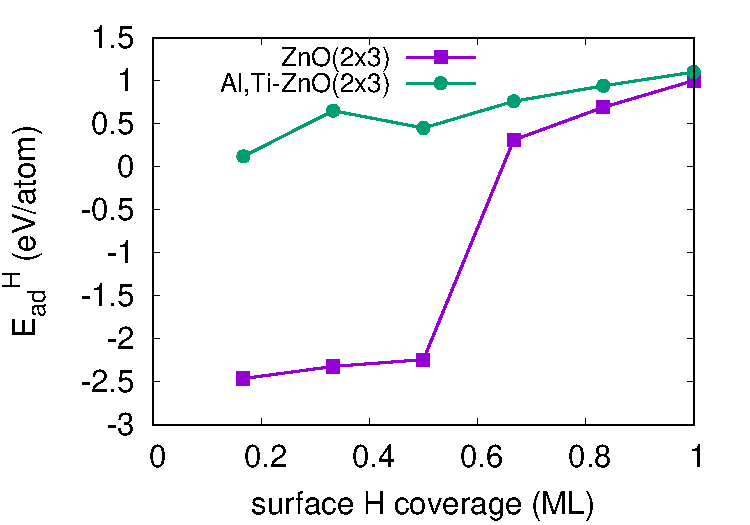
\includegraphics[width=0.45\linewidth]{Chap1/Eadh_2x3_H.pdf}}\label{Chap:ZnO_H:fig:2dop}
  \subfigure[]{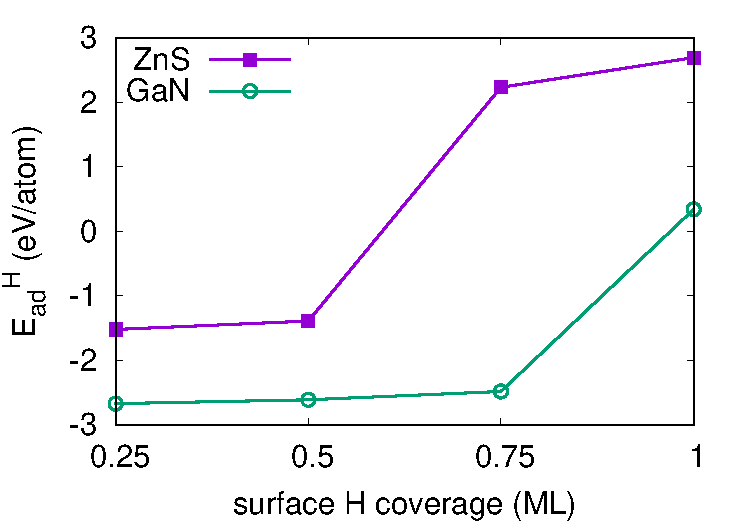
\includegraphics[width=0.45\linewidth]{Chap1/E_C_4.pdf}}\label{Chap:ZnO_H:fig:otherads}
\caption{(e) $E_{\textup{ad}}^{\textup{H}}$ on (2$\times$3) ZnO (000$\overline{1}$) surface with the co-existence of 1 Al substitutional dopant atom and 1 Ti substitutional dopant atom at bulk Zn sites. (a):$E_{\textup{ad}}^{\textup{H}}$ on (2$\times$2) zincblende ZnS ($\overline{1}$$\overline{1}$$\overline{1}$) and wurtzite GaN (000$\overline{1}$) surfaces with different $\theta_{\textup{H}}$. }
  \label{Chap:ZnO_H:fig:others}
\end{figure}
\endgroup

The electron counting model and Eq. \ref{eq3} can be used to explain the H adsorption strength on other polar semiconductor surfaces. For example, sulfur(S)-terminated ($\overline{1}$$\overline{1}$$\overline{1}$) surface of zincblende ZnS have the similar atomistic structure and valence electron configuration as those for wurtzite ZnO (000$\overline{1}$). As shown in Fig. \ref{Chap:ZnO_H:fig:otherads}, the dramatic decrease of H adsorption strength happens when $\theta_{\textup{H}}$ increases from $\frac{1}{2}$ to $\frac{3}{4}$ ML, the same as ZnO in Fig. \ref{Chap:ZnO_H:fig:Ead}. Moreover, for nitrogen(N)-terminated (000$\overline{1}$) surface of wurtzite GaN, because each N atom has 5 valence electrons and 4 Ga-N bonds, $\frac{8-5}{4}$ = 0.75 electron is required to saturate each N atom on (000$\overline{1}$) surface once the GaN bulk lattice is chopped into two surfaces along [0001] direction. According to Eq. \ref{eq3}, $N_{\textup{bond}}$ = 4, $V_{\textup{anion}}$ = 5, and $\theta_{\textup{dopant}}^i$ = 0 ML, so $\theta_{\textup{H}}^{\textup{c}}$ = $\frac{3}{4}$ ML . Therefore, $\theta_{\textup{H}}$ = $\frac{3}{4}$ ML, equivalent to 3 hydrogen atoms in the supercell of a (2$\times$2) GaN (000$\overline{1}$) surface, can transform all 4 surface N atoms from metallic to semiconductor states. Correspondingly, the hydrogen adsorption strength decreases dramatically when $\theta_{\textup{H}}$ increases from $\frac{3}{4}$ to 1 ML as shown in Fig. \ref{Chap:ZnO_H:fig:otherads}. 

\section{Conclusions}

In summary,  the coverage-dependent adsorption of hydrogen atoms on O-terminated (000$\overline{1}$) surface of wurtzite ZnO and other similar polar semiconductor surfaces behave differently than the counterparts on typical metal/alloy surfaces, where H adsorption strength usually decreases slightly and continuously (more positive values of $E_{\textup{ad}}^{\textup{H}}$ in Fig. \ref{Chap:ZnO_H:fig:Ead} ) with increasing H surface coverage \cite{pallassana1999theoretical,qi2012adsorbate}. The adsorption strength of individual H atom on these semiconductor surfaces strongly depends on hydrogen coverage and surface electronic structures. If the surface is in the metallic state, the hydrogen adsorption strength is so strong that the adsorption-dissociation reaction of a single H$_2$ molecule on this surface is highly exothermic at zero K ($E_{\textup{ad}}^{\textup{H}} < -2.0 $ eV in Eq. \ref{eq1}). If the surface is in semiconductor state, the hydrogen adsorption strength is so weak that the adsorption-dissociation reaction of a single H$_2$ molecule on this surface is endothermic at zero K ($E_{\textup{ad}}^{\textup{H}} > 0 $ in Eq. \ref{eq1}).  The surface can be transformed from metallic to semiconductor state by either hydrogen adsorption on the surface or dopant elements in bulk lattice in order to saturate unpaired electrons of anion elements on the top surface layer. The critical H surface coverage $\theta_{\textup{H}}^{\textup{c}}$ to induce such metal-semiconductor transition, which is also the equilibrium H coverage at many experimental conditions \cite{lin2007density,meyer2004first,lauritsen2011stabilization},  is determined by the classical electron counting model described in Eq. \ref{eq3} \cite{pashley1989electron}. This model is confirmed by our investigations of H adsorption on (000$\overline{1}$) surfaces of ZnO with a series of doping elements (Na, Mg, Al, Ti, Fe, Sn, etc.). When doping elements (such as Be, Mg, Na) have equal or less valence electrons than Zn, the critical H coverage will remain unchanged or increase to higher coverages. When doping elements (such as Al, Ti and V) have more valence electrons than Zn, the critical H coverage will decrease to lower coverages. When doping elements (such as Fe, Sn and Pb) have multiple common charge states, the behavior of the critical H coverage will become sophisticated but still follows the general electron counting rule.

This simple electron counting model can be applied to determine and manipulate the equilibrium surface adsorption configurations for H and other adsorbates on different semiconductor polar surfaces with chemical dopant elements. It is different than the d-band model that is widely used to understand trends of H adsorption strengths on different transition metal surfaces \cite{HAMMER95,Kibler05}. Since the driving force for surface reconstruction is also from the tendency to eliminate unpaired electrons and dangling bonds, the model can be used to identify the possible adsorbate and dopant configurations to obtain stable semiconductor surface structures \cite{Kaxiras87,pashley1989electron, Jacobs16ZnO}. It also suggests that the investigations of further adsorptions and depositions of other materials on these semiconductor surfaces should consider the coexistence of adsorbed H atoms at stable configurations. For example,  in many optoelectronic applications, ZnO and other semiconductor oxides are used as the substrate materials for metallic thin films, whose adhesion strengths on these substrates can be reduced significantly because of adsorbed H on substrate surfaces, resulting in thin-film dewetting and the formation of the undesired discontinued islands \cite{lin2007density,duriau2006growth}. This study provides a critical step to understand the substrate surface structures and adsorption characteristics for the further investigations on thin film qualities and optoelectronic properties.